\section{Bubble sort}
\subsection{Aim}
To perform bubble sort on 8-bit numbers

\subsection{Code}
\begin{lstlisting}
ORG 0000H

startaddr EQU 100H

MOV R0, #08H
MOV R1, #00H

MOV DPTR, #startaddr

DEC R0
MOV A, R0
MOV R1, A

OUTERLOOP:
	MOV A, R0
	MOV R2, A
	MOV DPTR, #startaddr
INNERLOOP:
	MOVX A, @DPTR
	MOV R3, A
	INC DPTR
	MOVX A, @DPTR
	SUBB A, R3
	JNC INNERLOOP_INCR

	MOVX A, @DPTR
	XCH A, R3
	MOVX @DPTR, A
	DEC DPL
	MOV A, R3
	MOVX @DPTR, A
INNERLOOP_INCR:
	DJNZ R2, INNERLOOP
OUTERLOOP_INCR:
	DJNZ R1, OUTERLOOP

EXIT:
	NOP
END
\end{lstlisting}

\subsection{Output}
\textbf{Input} 18H, 17H, 16H, 15H, 20H, 21H, 21H, 18H (at locations starting from \#100H on XDATA)\\
\textbf{Output} 15H, 16H, 17H, 18H, 18H, 20H, 21H, 21H\\
\begin{center}
	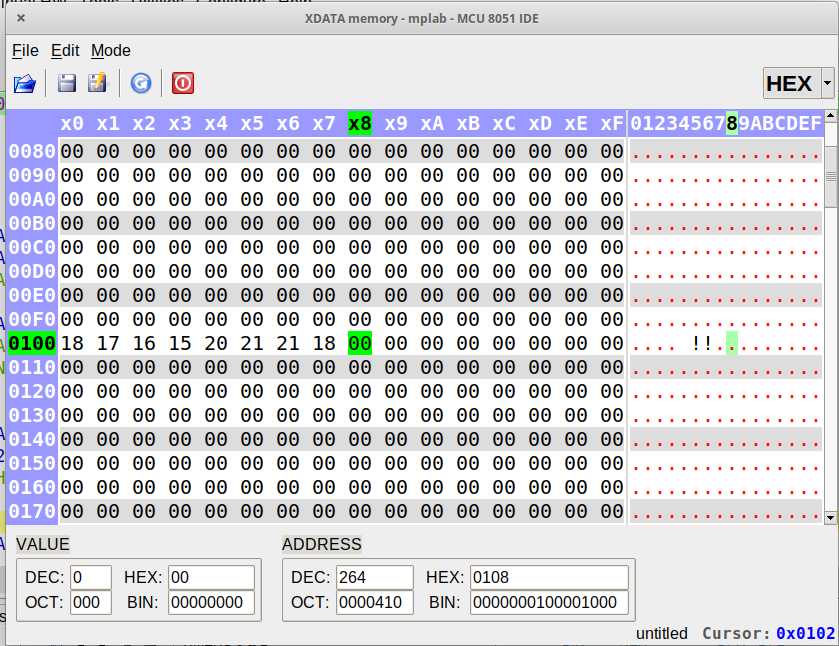
\includegraphics[width=\textwidth]{img/p30/ss1.png}
\end{center}
\begin{center}
	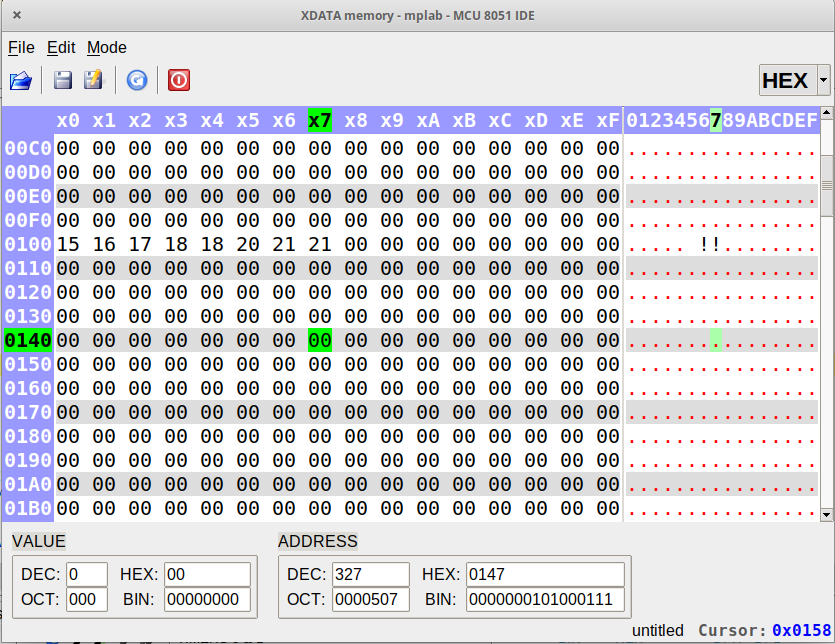
\includegraphics[width=\textwidth]{img/p30/ss2.png}
\end{center}


\subsection{Result}
Bubble sort was performed on an array was found on mcu8051ide